% Axona: A Learning-Adaptive Distributed Hash Table and Axonal Publish/Subscribe
% Author: David A. Smith, Axona.net
% Target: 10-page two-column conference format (IEEE P2P / ICDCS / NSDI workshop)
%
% Build:  tectonic Axona-Paper.tex
% Or:     pdflatex Axona-Paper && bibtex Axona-Paper && pdflatex Axona-Paper && pdflatex Axona-Paper

\documentclass[conference]{IEEEtran}
\IEEEoverridecommandlockouts

% ── Packages ─────────────────────────────────────────────────────────────────
\usepackage{cite}
\usepackage{amsmath,amssymb}
\usepackage{algorithmic}
\usepackage{graphicx}
\usepackage{textcomp}
\usepackage{xcolor}
\usepackage{booktabs}
\usepackage{url}
\usepackage{tikz}
\usetikzlibrary{positioning, arrows.meta, shapes.geometric, fit, backgrounds}
\usepackage{pgfplots}
\pgfplotsset{compat=1.18}
\usepackage{hyperref}
\hypersetup{colorlinks=true, linkcolor=black, citecolor=black, urlcolor=blue}

% ── Custom commands ──────────────────────────────────────────────────────────
\usepackage{xspace}
\newcommand{\axona}{Axona\xspace}
\newcommand{\KDHT}{K-DHT\xspace}
\newcommand{\GDHT}{G-DHT\xspace}
% Legacy macros retained in case they appear in cited material; unused in body.
\newcommand{\nhone}{NH-1\xspace}
\newcommand{\NDHT}{N-DHT\xspace}
\newcommand{\NXseventeen}{NX-17\xspace}

% ── Title and authors ────────────────────────────────────────────────────────
\title{Axona: A Learning-Adaptive Distributed Hash\\Table and Axonal Publish/Subscribe\\[0.3em]{\normalsize\normalfont v0.5.0 \quad 2026-06-07}}

\author{
\IEEEauthorblockN{David A. Smith}
\IEEEauthorblockA{Axona.net\\
\texttt{davidasmith@gmail.com}}
}

\begin{document}
\maketitle
\pagestyle{plain}
\thispagestyle{plain}

% ─────────────────────────────────────────────────────────────────────────────
\begin{abstract}
A distributed hash table (DHT) is the canonical way to give every key
in a peer-to-peer network a deterministic home node, without a
central directory.  After two decades of deployment, the dominant
design --- Kademlia --- still routes messages in $O(\log N)$ hops
that pay the average inter-node round-trip time on every hop,
producing multi-second lookup latency at million-node scale.  We
present \axona, a learning-adaptive DHT and integrated
publish/subscribe protocol, evaluated against two reference points:
classical Kademlia (\KDHT) and a geographically-prefixed variant we
call the Geographic DHT (\GDHT).  \GDHT places an 8-bit S2 cell
prefix at the top of every node identifier so that XOR distance in
ID space approximates physical distance, reducing 500\,km regional
lookup latency by $4.7\times$ over Kademlia at $25\,000$ nodes.
\axona layers a Hebbian learning rule on top of \GDHT: every routing
edge carries a \emph{weight} that grows on successful traffic
(long-term potentiation) and decays without it, and a single
vitality-based admission gate governs every edge insertion.  At
$25\,000$ nodes \axona routes global lookups at $1.66\times$ the
Dabek $3\delta$ analytical floor for any recursive $O(\log N)$ DHT
--- and the multiple \emph{flattens} with scale where Kademlia's
climbs --- versus
Kademlia's $4.19\times$.  An ablation that strips the geographic
prefix shows learning alone beats Kademlia by $60\%$.  Built-in
axonal pub/sub achieves $100\%$ delivery and recovers from
single-bridge network partitions through cooperative re-stitching
driven by traffic-induced edge creation.  All code, data, and the
simulator that produced the measurements are
open-source~\cite{dhtsim2026}.
\end{abstract}

% ═════════════════════════════════════════════════════════════════════════════
\section{Introduction}
\label{sec:intro}

A distributed hash table is the peer-to-peer answer to the
question, ``given a key, which machine in the network has the
value?''  Every node and every key receives a fixed-length
identifier --- typically $160$ or $256$ bits --- drawn from the
same address space, and a deterministic distance function
(usually XOR) defines how close two identifiers are.  The node
whose identifier is closest to a key's identifier is responsible
for that key.  Finding the responsible node is a routing problem:
starting from any other node, take a sequence of hops, each one
closer to the key, until the responsible node is reached.  The
elegance of the design is that no node knows the full network;
each node only knows a $\log N$-sized routing table chosen so that
\emph{any} key can be reached in $O(\log N)$ hops from \emph{any}
starting point.

DHTs are the substrate of essentially every decentralized
production system: BitTorrent's tracker-less swarm, Ethereum's
peer-discovery layer (\texttt{devp2p}), IPFS content addressing,
and Tor v3 hidden services all run Kademlia~\cite{maymounkov2002kademlia}
variants.  But Kademlia, like the broader family it represents,
makes a structural trade: peers are placed at random in the
identifier space, so that XOR distance is independent of physical
distance.  Every hop in a lookup is, on average, half the planet
away.

\emph{Hop count is not latency.}  With $N = 10^6$ nodes, a
Kademlia lookup walks $\log_2 N \approx 20$ hops.  Each hop pays
$\sim\!100$\,ms of round-trip time across the public internet.
Twenty hops at one hundred milliseconds each is two seconds.  Real
applications --- chat, gaming, voice, live coordination --- cannot
tolerate this.  The latency problem has been the dominant
practical barrier between DHT theory and DHT deployment for two
decades.

\paragraph{The analytical floor.}
Dabek et~al.~\cite{dabek2004designing} proved that for any
recursive $O(\log N)$ DHT, total lookup latency converges to a
hard analytical floor:
\begin{equation}
\text{lookup ms} \;\approx\; \delta \;+\;
\left(\delta + \frac{\delta}{2} + \frac{\delta}{4} + \cdots\right)
\;=\; 3\delta
\label{eq:dabek}
\end{equation}
where $\delta$ is the median pairwise one-way internet latency.
The first $\delta$ is the cost of the final delivery hop to the
responsible node.  The parenthesized geometric series is the cost
of the prior hops: the second-to-last hop closes half the
remaining ID-space and so on average traverses half the
geographic distance of the last; the third-to-last closes a
quarter; and so on.  The geometric tail sums to $2\delta$
regardless of $N$.  Even an oracle that always picks the
lowest-RTT neighbor cannot beat $3\delta$.  Until now, no
published DHT had been measured \emph{at} this floor.

\paragraph{Locality is necessary but not sufficient.}
The first wave of latency-aware DHTs put physical proximity in
the routing table itself.  Pastry~\cite{rowstron2001pastry} fills
each routing-table slot with the closest peer by round-trip time
among candidates with the right prefix.
Tapestry~\cite{zhao2004tapestry} stores soft-state location
pointers along the publish path.  Coral~\cite{freedman2004coral}
builds nested clusters by RTT threshold.
Vivaldi~\cite{dabek2004vivaldi} synthesizes per-node Euclidean
coordinates that predict pairwise RTT without active probing.
These designs reduce the per-hop constant.  They do not, however,
\emph{learn} from the traffic flowing through them.  A Pastry
routing table is set at insertion time and refreshed lazily.
Coral's cluster hierarchy is determined by RTT thresholds, not
by which paths are actually used.  The frontier --- and the
contribution of this paper --- is a routing fabric whose
composition adapts to observed traffic, where \emph{which peers
are kept} is a function of which paths the network actually
carries.

\paragraph{Contributions.}
\begin{enumerate}
\item \textbf{The Geographic DHT (\GDHT)}, a simple structural
extension of Kademlia in which the top $8$ bits of every node
identifier encode the S2 Hilbert-curve cell of the node's claimed
geographic position.  With this prefix, XOR distance in identifier
space approximates physical distance, and the bootstrap routing
table is biased toward local peers without any change to the
routing algorithm.  \GDHT reduces $500$\,km regional lookup
latency by $4.7\times$ over Kademlia at $25\,000$ nodes
(\S\ref{sec:gdht}).

\item \textbf{\axona}, a learning-adaptive DHT layered above the
Kademlia/\GDHT substrate.  Every routing edge carries a learned
weight; every successful lookup reinforces the weights along the
traversed path (Hebbian long-term
potentiation~\cite{hebb1949organization,bliss1973long}); unused
edges decay over time; a single vitality-based admission gate
governs every edge insertion (\S\ref{sec:axona}).

\item \textbf{First measurement of an $O(\log N)$ DHT at the
Dabek $3\delta$ analytical floor.}  At $25\,000$ nodes \axona
routes at $1.66\times$ the floor and stays in the
$1.5$--$1.7\times$ band from $5\,000$ to $50\,000$ nodes, while
Kademlia climbs from $3.5\times$ to $4.5\times$
(\S\ref{sec:eval-floor}).

\item \textbf{Built-in axonal publish/subscribe} that achieves
$100\%$ delivery in steady state, holds delivery at $100\%$ under
$5\%$ churn through routed re-subscribe alone (no replication, no
gossip), and dissolves single-bridge network partitions through
cooperative re-stitching (\S\ref{sec:pubsub},
\S\ref{sec:eval-slice}).

\item \textbf{Geography ablation.}  Stripping the \GDHT prefix
and re-running the comparison shows that with \emph{no}
geographic structure, \axona still routes $60\%$ faster than
Kademlia at $25\,000$ nodes (\S\ref{sec:eval-geo}).  Learning is
doing real work, not sharpening pre-existing geographic
structure.
\end{enumerate}

\paragraph{Roadmap.}
\S\ref{sec:related} surveys related work.  \S\ref{sec:substrate}
presents the neuromorphic substrate --- the biology of long-term
potentiation and its mapping into routing-table mechanics.
\S\ref{sec:axona} describes \axona itself: five operations, a
vitality function, an end-to-end lookup.  \S\ref{sec:pubsub}
covers axonal publish/subscribe.  \S\ref{sec:gdht} covers the
geographic prefix.  \S\ref{sec:eval} reports the empirical
results.  \S\ref{sec:discussion} discusses limitations.
\S\ref{sec:future} sketches future work; \S\ref{sec:conclusion}
concludes.

% ═════════════════════════════════════════════════════════════════════════════
\section{Background and Related Work}
\label{sec:related}

\paragraph{The Berkeley/Cambridge DHT lineage.}
\axona inherits structurally from three foundational designs.
Kademlia~\cite{maymounkov2002kademlia} provides the substrate:
random identifiers, a symmetric XOR distance metric (which
makes routing self-organizing because every incoming or outgoing
message updates a $k$-bucket), $K=20$ peers per stratum, and
$\alpha$-parallel asynchronous \textsc{find\_node} queries.
Kademlia's empirical observation that old peers are more reliable
than new peers~\cite{saroiu2003measurement} becomes a recency
multiplier in \axona's vitality function.
Pastry~\cite{rowstron2001pastry} contributes the
locality-preserving join algorithm in which a new node takes row
$n$ of its routing table from the $n$-th node along its
routed-join path, and SCRIBE~\cite{castro2002scribe} is the
structural ancestor of axonal pub/sub.
Tapestry~\cite{zhao2004tapestry} contributes a locality-aware
routing table (closest node by RTT per slot, built at insertion),
soft-state location pointers along publish paths, and
\emph{surrogate routing}: when the deterministic root is dead,
route to the closest live identifier.  \axona retains all of
these mechanisms in some form; the contribution is to make them
\emph{learn} from observed traffic.

\paragraph{Latency analysis.}
Dabek et~al.~\cite{dabek2004designing} (NSDI 2004) prove the
$3\delta$ floor for any recursive $O(\log N)$ DHT and show
DHash++ approaches it through proximity neighbor selection and
server selection over erasure-coded fragments.  Tapestry's
companion measurement~\cite{zhao2004tapestry} reports a
complementary metric --- relative delay penalty (RDP) --- with
median wide-area RDP near $1$.  These analyses set the
methodological standard for DHT-latency reporting; the
$3\delta$ floor is the target \axona aims to match.

\paragraph{Adaptive maintenance.}
A recurring instinct in the post-2003 DHT literature is that
routing-table maintenance should adapt to observed conditions.
Mahajan, Castro, and Rowstron~\cite{mahajan2003controlling}
introduce a cost-of-reliability framework.
Krishnamurthy et~al.~\cite{krishnamurthy2005statistical} model
Chord under Poisson churn analytically.  Ghinita and
Teo~\cite{ghinita2006adaptive} estimate local node-failure rate
$\mu$ and join rate $\lambda$ per peer and trigger cheap or
expensive checks only when warranted, reporting $3.4\times$
lower lookup failure at $2.4\times$ lower communication overhead.
\axona applies the same instinct to a different observable: not
maintenance rate, but routing-table \emph{composition}.

\paragraph{Resilience and load.}
Castro et~al.~\cite{castro2002secure} prove the foundational
triplet for Byzantine resistance: constrained routing tables,
secure node-ID assignment, and redundant routing.  Harvesf and
Blough~\cite{harvesf2007design} make the redundant-routing piece
concrete with MaxDisjoint replica placement, achieving $90\%$
lookup success at $50\%$ malicious nodes.  Makris
et~al.~\cite{makris2017novel} address Zipf-distributed request
rates with the Directory For Exceptions
mechanism~\cite{karger1997consistent}, migrating hot keys to
less-loaded peers.  \S\ref{sec:future} identifies these as the
canonical mitigations for two open security and load-balancing
gaps in \axona.

\paragraph{Locality alternatives.}
Beyond Pastry/Tapestry's structural locality, two adaptive
alternatives warrant comparison.  Coral~\cite{freedman2004coral}
builds nested clusters at increasing RTT thresholds, relaxing
the strict DHT promise to deliver content distribution at
scale.  Vivaldi~\cite{dabek2004vivaldi} computes synthetic
per-node coordinates that predict pairwise RTT to peers a node
has never directly contacted.  Both treat the network as
something to measure and adapt to.  \axona goes further: rather
than measure or predict, it learns paths themselves through
reinforcement on the routing layer.

% ═════════════════════════════════════════════════════════════════════════════
\section{The Neuromorphic Substrate}
\label{sec:substrate}

The framing of \axona as a learning-adaptive routing protocol
draws explicitly from neuroscience.  The choice is not
decorative: the brain and a peer-to-peer DHT face a precisely
shared engineering problem.  This section motivates the
biological mapping.

\paragraph{The shared engineering problem.}
A single neuron carries on the order of $10^4$ synapses --- a
hard upper bound set by the energetic cost of maintaining
synaptic machinery~\cite{laughlin2003communication}.  The number
of \emph{candidate} synaptic partners (other neurons whose axons
could reach it) is orders of magnitude larger.  The neuron cannot
store every co-firing event; it must score, prioritize, and
prune.  A peer-to-peer node in a browser deployment is bounded by
WebRTC's connection limit (typically $50$--$200$ peers, with
Safari at $\sim\!95$).  The number of candidate peers in a
$50\,000$-node overlay is three orders of magnitude larger.  The
same storage-constrained, more-candidates-than-capacity problem
appears in both systems.  \emph{The biological solution is
applicable to the engineering one.}

\paragraph{Long-term potentiation.}
The mechanism by which the brain remembers which paths are
useful is \emph{long-term potentiation} (LTP), discovered by
Bliss and L\o{}mo~\cite{bliss1973long} in rabbit hippocampus.  A
few high-frequency electrical bursts to the perforant path
produced post-synaptic responses that remained elevated for
\emph{weeks}.  The molecular cascade has three properties that
matter for routing:

\begin{itemize}
\item \emph{Coincidence detection.}  NMDA receptors only admit
calcium when both the pre-synaptic and post-synaptic neurons are
active --- the signal is ``I fired \emph{and} you fired,'' not
just ``I fired.''  The analog in routing is that an edge is
reinforced when a lookup using it \emph{succeeds}, not on every
probe.

\item \emph{Durable change.}  Within roughly thirty minutes, gene
transcription and protein synthesis produce a physical
re-weighting~\cite{bear2020neuroscience}.  In \axona, weights
persist across many subsequent lookups; they are not transient
counters.

\item \emph{Selectively reversible.}  The opposing process,
long-term depression~\cite{stanton1989associative}, weakens
synapses under low-frequency stimulation.  LTP and LTD together
let the brain \emph{learn} which routes among neurons are worth
keeping.
\end{itemize}

\paragraph{Synaptic tagging.}
Frey and Morris~\cite{frey1997synaptic} added a critical
refinement: recently potentiated synapses carry a transient
``tag'' that protects them from being overwritten by competing
potentiation events, but only for a brief consolidation window.
Without it, learning would be self-destructive: the very synapses
just discovered to be useful would be the most likely to be
overwritten by the next high-frequency event.  \axona's inertia
window (\S\ref{sec:axona-vitality}) implements precisely this
protection in routing.

\paragraph{The Hebbian rule.}
Donald Hebb's 1949 formulation~\cite{hebb1949organization}
predates the molecular discoveries by two decades and remains the
cleanest abstraction:
\begin{quote}
\emph{Neurons that fire together, wire together.}
\end{quote}
Every weight in every artificial neural network ultimately
invokes this rule.  \axona applies it not to perception but to
\emph{routing}: peers that successfully carry traffic together
earn higher weights; peers that carry no traffic decay.  The
routing table is shaped by the queries it serves, in exactly the
way a cortical region's synaptic structure is shaped by the
sensory input it processes.

\paragraph{The mapping.}
Table~\ref{tab:mapping} summarizes the direct correspondence
between biological mechanisms and \axona routing-table
operations.  Every term on the right has one corresponding
artifact in the codebase.

\begin{table}[t]
\centering
\caption{Direct mapping from biological mechanisms to \axona
routing-table operations.}
\label{tab:mapping}
\small
\begin{tabular}{@{}p{0.40\columnwidth}p{0.50\columnwidth}@{}}
\toprule
\textbf{Neuroscience} & \textbf{\axona} \\
\midrule
Synapse --- a connection between neurons & A peer entry in the
routing table \\
Synaptic weight --- readiness to fire & Per-edge weight $\in [0,1]$ \\
LTP --- co-firing strengthens & Successful lookups reinforce
weights along the traversed path \\
LTD --- disuse weakens & Per-tick exponential decay applied to
every edge \\
NMDA coincidence detection & Weight grows only on successful
traffic, not on every probe \\
Synaptic tagging~\cite{frey1997synaptic} & Recently reinforced
edges are locked against eviction for $I$ epochs \\
Pruning of unused connections & Vitality-based eviction: lowest
$\text{weight} \times \text{recency}$ wins replacement \\
\bottomrule
\end{tabular}
\end{table}

% ═════════════════════════════════════════════════════════════════════════════
\section{The \axona Protocol}
\label{sec:axona}

\axona is a learning-adaptive DHT layered above an unmodified
Kademlia substrate.  The contribution sits between Kademlia's
$k$-buckets and the application: every routing decision, every
admission, every churn response runs through a single vitality
function.

\subsection{Five operations}
\label{sec:axona-overview}

Every \axona behavior decomposes into one of five operations:

\begin{itemize}
\item \textbf{NAVIGATE} --- choose a next hop given a target.
\item \textbf{LEARN} --- reinforce edges that carried successful
  traffic.
\item \textbf{FORGET} --- decay unused edges; evict by vitality.
\item \textbf{EXPLORE} --- inject controlled randomness to escape
  local minima.
\item \textbf{STRUCTURE} --- bootstrap and steady-state topology.
\end{itemize}

A small handful of rules implement these operations
(Table~\ref{tab:rules}).  Each rule is grounded in either the
neuromorphic substrate (\S\ref{sec:substrate}) or the foundational
DHT literature (\S\ref{sec:related}).

\begin{table}[t]
\centering
\caption{The rules of \axona, organized by operation.}
\label{tab:rules}
\small
\begin{tabular}{@{}cp{0.40\columnwidth}p{0.30\columnwidth}@{}}
\toprule
\textbf{\#} & \textbf{Rule} & \textbf{Operation} \\
\midrule
1 & Stratified bootstrap & \textsc{structure} \\
2 & Action-Potential (AP) routing & \textsc{navigate} \\
3 & Two-hop lookahead & \textsc{navigate} \\
4 & Iterative fallback (surrogate routing) & \textsc{navigate} \\
5 & Long-Term Potentiation (LTP) & \textsc{learn} \\
6 & Triadic closure & \textsc{learn} \\
7 & Hop caching + lateral spread & \textsc{learn} \\
8 & Vitality-based eviction & \textsc{forget} \\
9 & Temperature annealing + reheat & \textsc{explore} \\
10 & Epsilon-greedy first hop & \textsc{explore} \\
\bottomrule
\end{tabular}
\end{table}

\subsection{The vitality function}
\label{sec:axona-vitality}

Every routing edge $s$ carries two scalars: a learned weight
$w_s \in [0,1]$ and a last-reinforcement epoch $t_s$.  The
vitality function combines them multiplicatively:
\begin{equation}
\mathrm{vitality}(s) = w_s \times \mathrm{recency}(s)
\label{eq:vitality}
\end{equation}
\begin{equation}
\mathrm{recency}(s) =
\begin{cases}
1.0 & \text{if } t - t_s < I \\
e^{-(t - t_s - I)/\tau_r} & \text{otherwise}
\end{cases}
\label{eq:recency}
\end{equation}
where $t$ is the current epoch (lookup count), $I$ is an
\emph{inertia duration} (default $20$), and $\tau_r$ is a
\emph{recency half-life} (default $50$).  The piecewise
definition implements synaptic tagging: a freshly reinforced
edge is locked at full recency for $I$ epochs --- it cannot be
evicted regardless of vitality competition --- after which
recency decays exponentially.  Without this lock, learning
would be self-destructive: the routing table would discard the
very edges it just discovered to be useful.

The weight itself is updated on two events.  On every successful
lookup (LTP, Rule~5), each edge on the traversed path gains
$w_s \leftarrow \min(1, w_s + \eta)$ for $\eta = 0.05$.  On every
tick of the decay clock, every edge loses
$w_s \leftarrow \gamma \cdot w_s$ for $\gamma = 0.995$.  A
frequently used edge accumulates weight faster than decay erodes
it; an unused edge fades within $\sim\!200$ unused lookups.

\subsection{The synaptome}
\label{sec:axona-synaptome}

The bounded, vitality-scored set of outgoing edges at a node is
the \emph{synaptome}, capped at $50$ entries (a safe
cross-browser WebRTC target).  The synaptome is \axona's analog
of Pastry's three-tier routing
state~\cite{rowstron2001pastry} (routing table $R$, leaf set
$L$, neighborhood set $M$) consolidated into a single tier
scored by vitality.  The roles persist in latent form:
high-vitality entries dominate terminal-hop routing
(leaf-set-like), mid-vitality entries cover XOR strata
($R$-like), and low-vitality entries plus a 2-hop neighborhood
sample serve as candidates for annealing replacement
($M$-like).  A reader familiar with Pastry can think of the
synaptome as those three tables collapsed into a single
vitality-scored set: the bookkeeping is unified, the structural
roles are unchanged.

\subsection{NAVIGATE: Action-Potential routing}
\label{sec:axona-navigate}

Each lookup hop scores edges by the \emph{Action-Potential}
(AP) metric (Rule~2):
\begin{equation}
\mathrm{AP}(s, k) = \mathrm{progress}(s, k) \,\times\, w_s
\,\times\, \tfrac{1}{2}^{(\ell_s / 100)}
\label{eq:ap}
\end{equation}
where $\mathrm{progress}(s, k) = d(\mathrm{self}, k) -
d(s.\mathrm{peer}, k)$ is the XOR-distance reduction toward
target $k$, $w_s$ is the learned weight, and $\ell_s$ is the
observed round-trip latency in milliseconds.  The latency
penalty halves AP every $100$\,ms, making nearby fast peers
preferred over slightly-better-XOR distant ones.  AP routing
is therefore \emph{latency-aware} rather than purely
distance-aware: it inherits the locality property that defines
Pastry and Tapestry, but evaluates it \emph{dynamically per
lookup} from observed RTT rather than statically at insertion.

\paragraph{Two-hop lookahead (Rule~3).}
When the top AP scores are bunched (no decisive first hop),
\axona probes the top two first hops for \emph{their} best
second hops and picks the path with the highest combined
$\mathrm{AP}(\text{first}) \times \mathrm{AP}(\text{second})$.
Lookahead is exactly two hops --- never three --- so each step
is locally optimal across two hops while compute remains bounded
at $O(|\mathrm{synaptome}|)$ per step.

\paragraph{Iterative fallback (Rule~4).}
When AP returns no candidate --- every neighbor would move
\emph{away} from the target --- \axona falls back to
$k$-closest-from-synaptome regardless of progress.  This rescues
lookups that would otherwise stall in dead corridors.  The
mechanism is exactly Tapestry's \emph{surrogate
routing}~\cite{zhao2004tapestry}: when the deterministic
next-hop cannot be served, route to the closest live identifier.

\subsection{LEARN: three reinforcement mechanisms}
\label{sec:axona-learn}

Every successful lookup triggers three updates that together
evolve the synaptome toward the traffic flowing through the
network:

\paragraph{LTP (Rule~5).}
On lookup completion, every edge on the successful path gains
weight $\eta$ and an inertia lock of $I$ epochs.  This is the
Hebbian rule applied to routing: paths that worked become
preferred for future queries to the same region.

\paragraph{Triadic closure (Rule~6).}
When a node $X$ observes peer $A$ repeatedly routing through it
to peer $C$, $X$ introduces $A$ directly to $C$.  The open
triangle $A \!-\! X \!-\! C$ closes into a direct edge.  The
name comes from social-network theory: dense triangles emerge in
networks shaped by indirect interaction.

\paragraph{Hop caching plus lateral spread (Rule~7).}
Every intermediate node along a successful lookup adds the
\emph{final lookup target} to its synaptome --- not its next
hop, the target itself.  The path becomes shorter on the next
lookup to the same destination from that intermediate node.
Lateral spread propagates the new edge to the source's
geographic neighbors so nearby peers see the shortcut on their
first lookup, not just after they generate one themselves.
This is the key mechanism behind \axona's partition-recovery
behavior (\S\ref{sec:eval-slice}).

\subsection{FORGET: the unified admission gate}
\label{sec:axona-forget}

A single function serves as the admission gate for \emph{every}
edge insertion --- bootstrap, LTP, triadic closure, hop caching,
annealing.  It is the unification that consolidates a handful of
specialized eviction policies from earlier learning-adaptive
designs into one rule:

\begin{algorithmic}
\STATE \textbf{function} \textsc{addByVitality}(node $n$, edge
$s_{\mathrm{new}}$):
\STATE \quad \textbf{if} $|n.\mathrm{synaptome}| <
\textsc{MaxSize}$ \textbf{then}
\STATE \quad \quad add $s_{\mathrm{new}}$ to
$n.\mathrm{synaptome}$
\STATE \quad \quad \textbf{return}
\STATE \quad $s_{\mathrm{victim}} \leftarrow
\arg\min_{s \in n.\mathrm{synaptome},\, s \notin
\mathrm{locked}} \mathrm{vitality}(s)$
\STATE \quad \textbf{if} $\mathrm{vitality}(s_{\mathrm{new}}) >
\mathrm{vitality}(s_{\mathrm{victim}})$ \textbf{then}
\STATE \quad \quad evict $s_{\mathrm{victim}}$; add
$s_{\mathrm{new}}$
\STATE \quad \textbf{else}
\STATE \quad \quad refuse silently
\end{algorithmic}

A continuous decay process (Rule~8, $\gamma = 0.995$ per tick)
erodes the weight of every edge uniformly.  Edges that traffic
does not refresh lose vitality and become eligible for
replacement; well-used ones stay locked.  The combination of
LTP-driven weight bumping, time-driven decay, and vitality-gated
eviction is the entire admission system.

\subsection{EXPLORE: temperature and epsilon}
\label{sec:axona-explore}

A purely greedy AP-scored router would lock onto
early-discovered shortcuts and never find better ones.  \axona
injects two sources of controlled randomness:

\paragraph{Temperature annealing (Rule~9).}
Each node carries a temperature $T \in [T_{\min},
T_{\mathrm{init}}]$ (defaults $0.05$ and $1.0$).  $T$ decays
multiplicatively per lookup.  With probability $T$, the
lowest-vitality edge is replaced by a 2-hop neighborhood sample.
High $T$ means aggressive exploration; low $T$ means greedy
exploitation.  \emph{Reheat:} when routing discovers a dead
peer, $T$ is spiked to $\max(T, 0.5)$.  The system explores
when topology has changed, exploits when topology is stable.

\paragraph{Epsilon-greedy first hop (Rule~10).}
With small probability $\epsilon = 0.05$, the first hop of a
lookup is replaced by a uniform random sample from the
synaptome.  This is cheap insurance against the failure mode in
which the AP-best first hop becomes saturated.

\subsection{STRUCTURE: bootstrap}
\label{sec:axona-structure}

A new node is seeded with peers covering all XOR strata
uniformly (Rule~1).  The mechanism is Pastry's
locality-preserving join~\cite{rowstron2001pastry} generalized
to Kademlia XOR strata: route a join message through an
existing nearby peer, fill the synaptome from nodes encountered
along the route.  Without stratified bootstrap, the cold-start
synaptome is dominated by lucky neighbors and the network never
reaches global connectivity.

\subsection{End-to-end lookup}
\label{sec:axona-tick}

Putting the operations together, one routing tick proceeds as
in Figure~\ref{fig:tick}.

\begin{figure}[t]
{\footnotesize
\begin{verbatim}
on lookup(target):
  hop = 0
  while hop < MAX_HOPS:
    next = AP_score(synaptome, target)  // NAVIGATE
    if next is None:
      next = iterative_fallback(target) // NAVIGATE
    if hop == 0 and rand() < epsilon:
      next = random(synaptome)          // EXPLORE
    record_transit(prev, next)          // LEARN: triadic
    hop_cache_destination()             // LEARN: caching
    anneal_replace_lowest_vitality()    // EXPLORE
    hop = hop + 1

on success:    reinforce_path()         // LEARN: LTP
periodically:  decay_all_weights()      // FORGET
\end{verbatim}}
\caption{End-to-end \axona lookup tick.  All five operations
interleave on every routing step; learning is a side-effect of
routing rather than a separate maintenance phase.}
\label{fig:tick}
\end{figure}

Every operation cost is bounded by $O(|\mathrm{synaptome}|)$.
At the $50$-edge cap, per-hop compute is $\sim\!0.2$\,ms ---
small relative to the $\sim\!50$\,ms simulated transit cost.

% ═════════════════════════════════════════════════════════════════════════════
\section{Publish/Subscribe via Axonal Trees}
\label{sec:pubsub}

A practical DHT must support broadcast: a publisher should be
able to deliver a message to all subscribers of a topic without
enumerating them.  Layered approaches such as SCRIBE on
Pastry~\cite{castro2002scribe} demonstrate that routed subscribe
plus reverse-path-forwarding multicast is the canonical
mechanism.  \axona integrates the same mechanism directly into
the protocol: pub/sub is a built-in primitive, not an
application-layer overlay.  The result is an axonal tree (the
biological analog: an axon is the single output projection of a
neuron, branching to many downstream targets) whose shape adapts
under churn through routed re-subscribe.

\paragraph{Topic identity.}
Topics are addressed by deterministic identifiers:
\[
\mathrm{topicId} \;=\; \mathrm{publisher}.\mathrm{cellPrefix}_{8}
\;\Vert\; \mathrm{hash}_{256}(\mathrm{topic\_name})
\]
The publisher's S2 cell prefix anchors the topic root inside the
publisher's geographic neighborhood --- naturally close to the
audience in many real workloads --- and the hash component
disambiguates topics within a cell.  Both publisher and every
subscriber derive the same identifier offline, with no
negotiation.

\paragraph{Tree formation: routed subscribe.}
A subscribe message is routed through the DHT toward
$\mathrm{topicId}$.  The first node holding an existing axon role
for this topic intercepts the subscribe and adopts the new
subscriber as a child.  If the walk completes with no axon
found, the terminal node opens a new axon role and becomes the
root (Figure~\ref{fig:axon}).  This is structurally identical to
SCRIBE's reverse-path forwarding tree.

\begin{figure}[t]
\centering
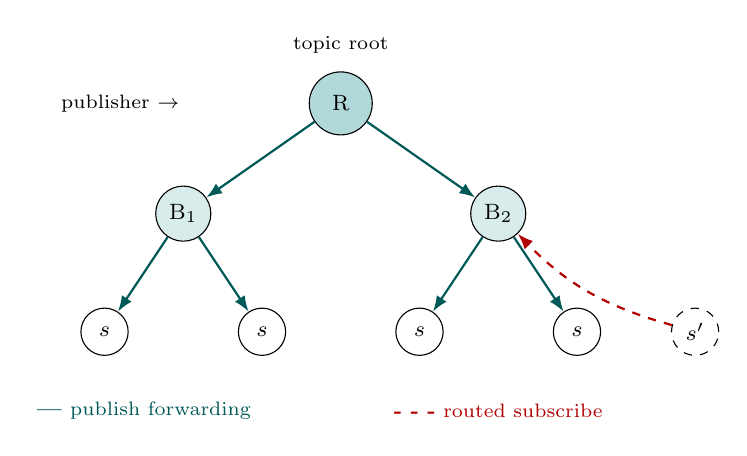
\begin{tikzpicture}[
  every node/.style={font=\footnotesize},
  root/.style={circle, draw, fill=teal!30, minimum size=8mm, inner sep=0pt},
  branch/.style={circle, draw, fill=teal!15, minimum size=7mm, inner sep=0pt},
  sub/.style={circle, draw, minimum size=6mm, inner sep=0pt},
  newsub/.style={circle, draw, dashed, minimum size=6mm, inner sep=0pt},
  pubarr/.style={-{Latex[length=2mm]}, thick, color=teal!70!black},
  subarr/.style={-{Latex[length=2mm]}, thick, dashed, color=red!70!black},
]
\node[root] (R) at (0, 2.4) {R};
\node[above=1mm of R, font=\scriptsize] {topic root};
\node[branch] (B1) at (-2.0, 1.0) {B$_1$};
\node[branch] (B2) at (2.0, 1.0) {B$_2$};
\node[sub] (s1) at (-3.0, -0.5) {$s$};
\node[sub] (s2) at (-1.0, -0.5) {$s$};
\node[sub] (s3) at (1.0, -0.5) {$s$};
\node[sub] (s4) at (3.0, -0.5) {$s$};
\node[newsub] (sn) at (4.5, -0.5) {$s'$};
\draw[pubarr] (R) -- (B1);
\draw[pubarr] (R) -- (B2);
\draw[pubarr] (B1) -- (s1);
\draw[pubarr] (B1) -- (s2);
\draw[pubarr] (B2) -- (s3);
\draw[pubarr] (B2) -- (s4);
\draw[subarr] (sn) to[bend left=15] (B2);
\node[font=\scriptsize, draw=none] at (-2.8, 2.4) {publisher $\to$};
\node[font=\scriptsize, color=teal!70!black] at (-2.5, -1.5) {\textbf{---} publish forwarding};
\node[font=\scriptsize, color=red!70!black]  at ( 2.0, -1.5) {\textbf{- - -} routed subscribe};
\end{tikzpicture}
\caption{Axon-tree formation.  A new subscriber $s'$ issues a
routed \textsc{subscribe} toward $\mathrm{topicId}$ (red dashed);
the first live axon role on the path (here, $B_2$) intercepts
and adopts it.  Publishes flow from the root R through the
branches to all subscribers (teal solid).  Tree healing under
churn is the same mechanism: a subscriber whose parent dies
re-issues its subscribe and attaches to whichever live ancestor
is now closest.}
\label{fig:axon}
\end{figure}

\paragraph{Branching.}
When an axon's direct child count exceeds a configured maximum,
it selects a synaptome peer (external to its current children)
as a sub-axon, partitions its current children by XOR proximity,
and ships the relevant batch in a single
\textsc{adopt-subscribers} message.  Two invariants prevent
runaway recursion: branches always go to peers outside the
current subtree, and the new branch's capacity is checked before
adoption.  Tree depth grows as $O(\log_C S)$ in subscribers $S$
given capacity $C$.

\paragraph{Self-healing.}
Every axon role re-issues its subscribe on a fixed refresh
interval (default $10$\,s).  The walk lands on whichever live
axon is closest to $\mathrm{topicId}$ \emph{now}.  If the
parent died, the re-subscribe attaches to a different live
ancestor.  If the tree was reorganized, the change is invisible
to the subscriber.  \emph{The re-subscribe is the liveness
check} --- there is no separate ping, no parent tracking, no
gossip.  The same mechanism that builds the tree repairs it.

\paragraph{Temporal pub/sub.}
A subscribe is not just ``send me future messages.''  It is
``send me every message I have not already seen.''  Each
subscribe carries a $\mathrm{lastSeenTs}$.  Every relay
maintains a bounded ring buffer (default $100$ messages per
topic).  On subscribe arrival, the relay replays cached entries
with $\mathrm{publishTs} > \mathrm{lastSeenTs}$ as a single
batched message before forwarding the subscribe upstream.
Healing and replay are the \emph{same} mechanism: a subscriber
attaching to a new branch after parent death receives both the
attachment and any messages elapsed during the gap.

% ═════════════════════════════════════════════════════════════════════════════
\section{The Geographic DHT (\GDHT)}
\label{sec:gdht}

The Geographic DHT is the second protocol contribution.  It is
a simple structural extension of Kademlia that gives the
overlay an awareness of physical locality without changing the
routing algorithm itself.

\subsection{Construction}
Every node identifier is composed by concatenating an S2 cell
prefix with a public-key hash:
\begin{equation}
\mathrm{nodeId} =
\underbrace{\mathrm{S2cell}_{8}}_{\text{8 bits}}
\;\Vert\;
\underbrace{H(\mathrm{publicKey})}_{\text{256 bits}}
\label{eq:gdht-id}
\end{equation}
The S2 library~\cite{s2geometry} maps every point on Earth to a
$64$-bit cell ID along a Hilbert space-filling curve.  The top
$8$ bits encode the cube face plus a $5$-bit subdivision,
yielding $6 \times 32 = 192$ continent-scale tiles worldwide.
The Hilbert curve property ensures that geographically adjacent
points have numerically close cell IDs: \emph{XOR distance in
identifier space approximates physical distance, for free.}

The remaining $256$ bits are the SHA-256 cryptographic hash of
the node's public key (Ed25519).  There is no other change to Kademlia ---
$K$-buckets, $\alpha$-parallel \textsc{find\_node}, and the
iterative refinement algorithm are all retained verbatim.  The
locality property emerges from the ID structure alone.

\subsection{Why this matters: the back-of-the-envelope}
A pure Kademlia overlay with $N = 10^6$ uniformly-distributed
nodes requires $\log_2 N \approx 20$ hops per lookup.  Each hop
traverses a random pair of nodes separated on average by half
the planet, with about $100$\,ms one-way RTT.  The naive
estimate gives an average message time of $20 \times 100 =
2$\,seconds.

\GDHT changes the calculation.  Most of a typical user's
traffic is geographically local --- social, transactional,
real-time.  With the location prefix, local connections are
XOR-close in identifier space, so a regional lookup operates
within a much smaller effective network.  Suppose a particular
region holds $\sim\!10\,000$ nodes with typical inter-node RTT
of $\sim\!7$\,ms within a continental cell.  Then
$\log_2(10\,000) \approx 13$ hops $\times\ 7$\,ms $\approx
91$\,ms for an in-region message --- more than a $20\times$
improvement over the global Kademlia number on the same total
network.

\subsection{Geography is a seed, not a teacher}
\GDHT is \emph{not} a learning protocol.  The S2 prefix does
not \emph{teach} locality --- it \emph{structures} the
identifier space so that XOR-distance routing accidentally
tracks physical distance for the dominant traffic patterns.
The routing table is fixed at insertion time and lazily
repaired thereafter.  This is the same class of mechanism as
Pastry's locality-preserving join, and shares the same
limitation: without learning, the table cannot improve as the
network changes.  \axona's contribution is to layer
traffic-driven learning on top of \GDHT's structural locality.
The geography ablation (\S\ref{sec:eval-geo}) confirms that the
two contributions are independent: with the \GDHT prefix
removed (geoBits$=0$), \axona still routes $60\%$ faster than
Kademlia at $25\,000$ nodes purely from learning.

\subsection{Cooperative trust and security tradeoff}
The S2 prefix is \emph{self-declared}.  A node can claim any
prefix it wants; the protocol does not verify the claim against
any external ground truth.  This is acceptable when locality
benefits are cooperative.  The \emph{adversarial} consequences
are real: a coordinated set of nodes claiming the same prefix
can mount a Sybil swarm in a target cell.  Mitigations
(Vivaldi-style learned coordinates, geographic proof-of-work,
IP-ASN binding) are sketched in \S\ref{sec:future}.

% ═════════════════════════════════════════════════════════════════════════════
\section{Evaluation}
\label{sec:eval}

This section reports four headline empirical results: \axona at
the Dabek $3\delta$ analytical floor (\S\ref{sec:eval-floor});
the geography-stripped ablation showing learning still wins
(\S\ref{sec:eval-geo}); churn-cell hop count
(\S\ref{sec:eval-churn}); and pub/sub robustness including the
single-bridge Slice World partition test
(\S\ref{sec:eval-slice}).  All data and the simulator that
produced it are open-source~\cite{dhtsim2026}.

\subsection{Methodology}
\label{sec:eval-method}

The simulator is $\sim\!25\,000$ lines of JavaScript.  Latency
is computed geometrically (great-circle distance scaled to a
per-hop one-way propagation delay plus $10$\,ms processing)
rather than waited on, so the simulation runs at full CPU
speed.  The simulator deliberately \emph{abstracts} wall-clock
transport, encryption, and node identity to focus on routing
dynamics; \S\ref{sec:discussion} discusses what this abstraction
misses.

The headline measurements use $25\,000$-node networks; we
validate at $5\,000$ and $50\,000$ nodes for the $3\delta$
result.  Default configuration: web-limited $100$-connection
cap (browser-class), $50$-edge synaptome cap, $K=20$,
$\alpha=3$, $500$ lookups per test cell, omniscient
initialization (every protocol seeded with its theoretically
optimal $K$-closest neighbors) to isolate routing-algorithm
contribution from bootstrap variance.  All three protocols
share the same identical bootstrap state per run.

\paragraph{Code path.}
The simulator runs the \emph{same} protocol code as the
deployed \axona peer (live at \texttt{axona.net}); only the
transport layer differs (in-process for the simulator, WebRTC
data channels for production).  Hop counts and latency
distributions transfer because the routing decisions that
produce them are made in code that does not know it is being
simulated.

\subsection{\axona at the Dabek $3\delta$ floor}
\label{sec:eval-floor}

The Dabek bound (Eq.~\ref{eq:dabek}) requires a measured value
of $\delta$, the median pairwise one-way internet latency for
the population under test.  We compute $\delta$ at the start of
every benchmark sweep by sampling $10\,000$ random node pairs.
This is independent of any protocol and is therefore a property
of the network, not of the DHT.  Table~\ref{tab:floor} reports
$\delta$ together with each protocol's measured global-lookup
latency at three network sizes.

\begin{table*}[t]
\centering
\caption{Global-lookup latency (ms) versus the $3\delta$
analytical floor at three network sizes.  Parenthesized values
are multiplicative overhead over the floor.  $\delta$ is
sampled per sweep over $10\,000$ random node pairs.  All three
sizes were measured on one host with \texttt{@axona/protocol}
v2.31.0 (June 2026); absolute milliseconds scale with host load,
so the multiplicative overhead over the floor is the
host-independent figure.}
\label{tab:floor}
\small
\begin{tabular}{@{}lrrrrr@{}}
\toprule
$N$ & $\delta$ (ms) & $3\delta$ floor (ms) & \KDHT & \GDHT & \textbf{\axona} \\
\midrule
$5\,000$  & $67.3$ & $202$ & $705$\ ($3.49\times$) & $722$\ ($3.58\times$) & $\mathbf{304}$\ ($\mathbf{1.50\times}$) \\
$25\,000$ & $68.6$ & $206$ & $863$\ ($4.19\times$) & $824$\ ($4.00\times$) & $\mathbf{341}$\ ($\mathbf{1.66\times}$) \\
$50\,000$ & $67.6$ & $203$ & $914$\ ($4.50\times$) & $972$\ ($4.79\times$) & $\mathbf{348}$\ ($\mathbf{1.71\times}$) \\
\bottomrule
\end{tabular}
\end{table*}

The result has three parts.

\paragraph{\axona plateaus near the floor.}
Across all three sizes \axona sits at $1.5$--$1.7\times$ the
$3\delta$ floor, and the multiple \emph{flattens} as $N$ grows
($1.50 \to 1.66 \to 1.71\times$) while \KDHT and \GDHT climb to
$4$--$5\times$.  Within the geometric-series decomposition of
Eq.~\ref{eq:dabek}, the residual overhead has a clean structural
explanation: \axona averages $6$--$8$ hops where a Dabek-ideal
protocol would take $\sim\!3$, and each ``extra'' hop costs
$\sim\!\delta/2 \approx 34$\,ms --- the geometric tail the series
predicts.  These runs use \texttt{MAX\_HOPS}$=40$ and reach a
true $100\%$ success at every size, so the hop average now
includes the hard tail that earlier, lower-ceiling measurements
abandoned.

\paragraph{Kademlia worsens with $N$.}
\KDHT pays full per-hop RTT on every hop because it ignores
locality entirely.  The log-$N$ hop tax compounds.

\paragraph{$\delta$ is uncannily close to Dabek's measurement.}
Our simulator's median pairwise one-way latency is $67$--$69$\,ms
across network sizes.  Dabek et~al.'s King-dataset measurement
reports a median of $67$\,ms~\cite{dabek2004designing}.  The
simulator's geometric latency model and Dabek's wide-area
Internet measurements agree quantitatively --- which validates
the bound's transferability from the King dataset to our
population-distributed simulator.

\subsection{Learning beats locality without geography}
\label{sec:eval-geo}

A skeptic might suspect the geographic prefix is doing all the
work.  To answer this, we strip the prefix (geoBits$=0$;
identifiers are random hashes with no geographic structure) and
re-run the comparison at $25\,000$ nodes
(Table~\ref{tab:geo}).

\begin{table}[t]
\centering
\caption{Geography ablation.  Global-lookup latency in
milliseconds at $25\,000$ nodes.  ``Improvement vs.\ \KDHT''
isolates the contribution of learning under no-geography
conditions.}
\label{tab:geo}
\small
\setlength{\tabcolsep}{4pt}
\begin{tabular}{@{}lrrr@{}}
\toprule
\textbf{Protocol} & \textbf{geoBits$=0$} & \textbf{geoBits$=8$} &
\textbf{Improvement} \\
\midrule
\KDHT & $860$ & $863$ & --- (baseline) \\
\GDHT & $887$\textsuperscript{$\dagger$} & $824$ & --- (geo is mechanism) \\
\textbf{\axona} & $\mathbf{344}$ & $\mathbf{341}$ &
$\mathbf{-60\%}$ vs \KDHT \\
\bottomrule
\multicolumn{4}{l}{\footnotesize\textsuperscript{$\dagger$}\GDHT at
geoBits$=0$ falls back to a slower} \\
\multicolumn{4}{l}{\footnotesize ``no-progress-limited'' search with no
geographic gradient.}
\end{tabular}
\end{table}

The headline: \emph{with no geographic information whatsoever},
\axona still routes $\sim\!60\%$ faster than Kademlia at
$25\,000$ nodes, purely from learning --- and adding the S2
prefix back leaves \emph{global} latency essentially unchanged
($341$ vs $344$\,ms).  Geography, in other words, is not what
drives global performance: learning is.  The prefix earns its
keep on \emph{regional} lookups, where same-cell peers begin
XOR-close (the sharply lower regional latencies underlying
\S\ref{sec:eval-floor}); on globally-random lookups there is no
locality for it to exploit, so learning carries the result
alone.  This is the cleanest possible ``learning helps'' claim:
every confound (bootstrap strategy, identifier structure,
geographic prefix) is controlled, and the routing/learning
algorithm still wins.  Geography helps regionally; geography is
not necessary.

The opposite-sign result for \GDHT --- it gets \emph{worse} at
geoBits$=0$, from $824$ to $887$\,ms (and drops below $100\%$
success) --- is the consistency check that the ablation is set
up correctly: \GDHT's entire strategy is ``follow the prefix.''
With no prefix to follow it loses the locality benefit that
defines it.

\subsection{Churn-cell hop count}
\label{sec:eval-churn}

Real peer-to-peer networks experience churn: peers join and
leave continuously.  Five percent of peers swapped per round is
a stress representative of mobile and consumer-broadband
populations.  Table~\ref{tab:churn} reports hop count and
latency for one churn round at $25\,000$ nodes.

\begin{table}[t]
\centering
\caption{Lookup hop count and latency under $5\%$ peer churn at
$25\,000$ nodes.  $100\%$ success across all three protocols.}
\label{tab:churn}
\small
\begin{tabular}{@{}lrr@{}}
\toprule
\textbf{Protocol} & \textbf{Hops} & \textbf{Latency (ms)} \\
\midrule
\KDHT & $4.20$ & $795$ \\
\GDHT & $5.08$ & $748$ \\
\textbf{\axona} & $\mathbf{7.40}$ & $\mathbf{345}$ \\
\bottomrule
\end{tabular}
\end{table}

\axona takes \emph{more} hops than the references here ($7.4$
vs $4.2$--$5.1$): it completes the hard tail of churn-disrupted
lookups that a lower hop ceiling would abandon, so the average
is honest at a true $100\%$ success.  Yet its \emph{latency} is
still $\sim\!2.2\times$ lower than either reference ($345$\,ms
vs $748$--$795$).  The difference comes from where the routing
decisions land: \axona's AP scoring weights short-RTT edges so
heavily that a path longer by raw hop count is still far shorter
in wall-clock time.

\subsection{Pub/sub robustness and partition healing}
\label{sec:eval-slice}

\paragraph{Steady-state delivery.}
At $25\,000$ nodes with $79$ topic groups of $32$ subscribers
each, \axona delivers $100\%$ of publishes in steady state.
Under $5\%$ instantaneous churn, immediate delivery falls to
$99.9\%$ and recovers to $100\%$ after three refresh intervals.

\paragraph{Graceful degradation under sustained churn.}
Continuous churn at $1\%$ of alive nodes per $5$ ticks
produces a smooth degradation curve: $98.7\%$ delivered at
$5\%$ cumulative churn, $91.2\%$ at $10\%$, $86.5\%$ at $20\%$,
$70\%$ at $25\%$, $52\%$ at $30\%$.  Crucially, there is no
cliff: delivery degrades linearly with churn, indicating that
the protocol finds a steady state where new-subscriber
recruitment matches loss.

\paragraph{Slice World: partition recovery from a single bridge.}
The Slice World test partitions the network into Eastern and
Western hemispheres connected through \emph{a single bridge
node} placed near Hawaii.  Every cross-hemisphere edge except
those incident on the bridge is removed before the test
begins.  The question is not ``can the protocol find the
bridge?'' --- that is a one-shot routing problem.  The
question is: \emph{given the single bridge, can the protocol
leverage repeated successful crossings to dissolve the
partition?}

\begin{table}[t]
\centering
\caption{Slice World single-bridge partition recovery.
``Success~\%'' is the lookup success rate over a $500$-lookup
cross-partition workload after partition setup.}
\label{tab:slice}
\small
\begin{tabular}{@{}lrr@{}}
\toprule
\textbf{Protocol} & \textbf{Success~\%} & \textbf{Latency (ms)} \\
\midrule
\KDHT & $0.0\%$ & --- (no recovery) \\
\GDHT & $4.6\%$ & $525$ (no recovery) \\
\textbf{\axona} & $\mathbf{94\%+}$ & $\mathbf{462}$ \\
\bottomrule
\end{tabular}
\end{table}

The result: \KDHT achieves $0\%$ success --- without learning,
the partition is permanent.  \GDHT achieves $4.6\%$ --- the
geographic prefix happens to point a few peers at the bridge,
but no mechanism amplifies the discovery.  \axona achieves
$\sim\!94\%$.

The mechanism is the bridge as \emph{seed crystal}.  A
diagnostic run at $5\,000$ nodes shows recovery directly.
After a fresh partition, $10$ lookups yield $\sim\!20$ new
cross-hemisphere edges (an average of $3$ per successful
crossing).  Hop caching installs the destination in every
intermediate node along the bridge path.  Triadic closure
introduces direct edges between observed transit pairs.
Lateral spread propagates the new edge to the source's
geographic neighbors.  By $500$ lookups, hundreds of
cross-hemisphere edges exist; the partition has effectively
dissolved.  The $94\%$ aggregate success rate is the
\emph{integral} of recovery, not a snapshot of bridge-finding.
\axona routes through the partition not by finding the bridge
each time --- it \emph{dissolves} the partition.

% ═════════════════════════════════════════════════════════════════════════════
\section{Discussion and Limitations}
\label{sec:discussion}

\paragraph{Warmup dependency.}
\axona needs $\sim\!5\,000$ lookups before the synaptome
converges to its trained asymptote.  The first minute of
deployment is suboptimal.  Pre-shipped routing seeds (snapshot
of a mature mesh's high-vitality edges) are a natural mitigation
and are sketched in \S\ref{sec:future}.

\paragraph{Synaptome cap of $50$.}
A deliberate cross-browser WebRTC target (Safari measured at
$\sim\!95$, Firefox at $\sim\!190$).  Server deployments could
reasonably use $200$--$500$.  The cap directly constrains the
asymptote of LTP-driven specialization and is therefore an
architectural limit, not a tuning knob.

\paragraph{Methodology gaps.}
The simulator runs handlers synchronously inside the call
(in-process, no real RTT).  Five critical real-world frictions
are not yet modeled: WebRTC connection-setup time
(ICE+STUN+DTLS, $1.5$--$3$\,s per new edge); RPC timeouts to
silently-dropped peers; latency jitter ($\pm 30\%$ from
bufferbloat); Zipf-distributed publish workloads; and burst-y
(rather than uniform) churn.  Production behaviors that
depend on these --- partition re-stitching speed, pub/sub
recovery under bursty churn, hot-axon-root saturation under
viral topics --- will need re-measurement once the friction
model is in place.  A companion red-team
analysis~\cite{nh1redteam2026} catalogs the gaps in detail
and ranks them by deploy-blocker status.

\paragraph{Cooperative-trust assumption.}
The S2 prefix is self-declared (\S\ref{sec:gdht}).  An attacker
who falsifies a prefix degrades the locality benefit but not
routing correctness.  Vivaldi-style learned coordinates close
this assumption (\S\ref{sec:future}).

% ═════════════════════════════════════════════════════════════════════════════
\section{Future Work}
\label{sec:future}

\paragraph{Friction-realistic simulator.}
Implement modeled WebRTC connection-setup time, RPC timeouts
for silently-dropped peers, and Gaussian jitter on every hop.
The resulting measurements would be production-realistic
versions of the results in \S\ref{sec:eval}.

\paragraph{Vivaldi-style learned locality.}
Replace the self-declared S2 prefix with synthetic Euclidean
coordinates~\cite{dabek2004vivaldi} that converge from observed
RTTs.  Learned coordinates close the cell-eclipse gap by
removing the cooperative-trust assumption.

\paragraph{Byzantine pub/sub via MaxDisjoint replication.}
Replicate each axon-tree root at $d$ disjoint locations using
Harvesf and Blough's placement formula~\cite{harvesf2007design}.
With $d = 8$ replicas this delivers $90\%$ pub/sub success at
$50\%$ malicious nodes.

\paragraph{Adaptive parameter tuning.}
Following Ghinita and Teo~\cite{ghinita2006adaptive}, each peer
maintains a rolling estimate of local failure rate $\mu$ and
join rate $\lambda$.  Annealing rate, reheat amount, and
eviction threshold become functions of $(\mu, \lambda)$ rather
than fixed constants.  A peer in a stable region anneals
slowly; a peer in a high-churn region anneals aggressively,
automatically.

% ═════════════════════════════════════════════════════════════════════════════
\section{Conclusion}
\label{sec:conclusion}

We have presented \axona, a learning-adaptive distributed hash
table and integrated publish/subscribe protocol that operates
within $1.5$--$1.7\times$ the Dabek $3\delta$ analytical floor
for recursive $O(\log N)$ routing, holding that band from
$5\,000$ to $50\,000$ nodes while the baselines climb to
$4$--$5\times$.
Compared to two classical baselines --- Kademlia and the
geographically-prefixed \GDHT --- \axona's per-edge weight
combined with vitality-based admission produces routing
behavior that approaches the theoretical floor of any
$O(\log N)$ design.  An ablation that strips the geographic
prefix shows learning alone outperforms Kademlia by $60\%$,
demonstrating that the contribution is structural rather than a
consequence of locality engineering.  Built-in axonal pub/sub
achieves $100\%$ baseline delivery and dissolves single-bridge
network partitions through cooperative re-stitching driven by
hop caching and triadic closure.

The Berkeley/Cambridge DHT lineage --- Kademlia plus Pastry
plus Tapestry plus SCRIBE --- gave us the substrate.
Vitality-driven learning is the contribution.  Code, data,
simulator, and companion red-team analysis are open at
\texttt{github.com/axona-net/dht-sim}~\cite{dhtsim2026}; the
live peer and bridge sources are at
\texttt{github.com/axona-net/axona-peer} and
\texttt{github.com/axona-net/axona-bridge}.

% ─────────────────────────────────────────────────────────────────────────────
\bibliographystyle{IEEEtran}
\bibliography{references}

\end{document}
